\input{mmd6-article-leader}
\def\mytitle{Guidance, Navigation, and Control Concept}
\def\myauthor{}
\def\mydate{}
\input{mmd6-article-begin}

\section{Frames of Reference}
\label{framesofreference}

\subsection{Robot Frame of Reference}
\label{robotframeofreference}

\begin{figure}[htbp]
\centering
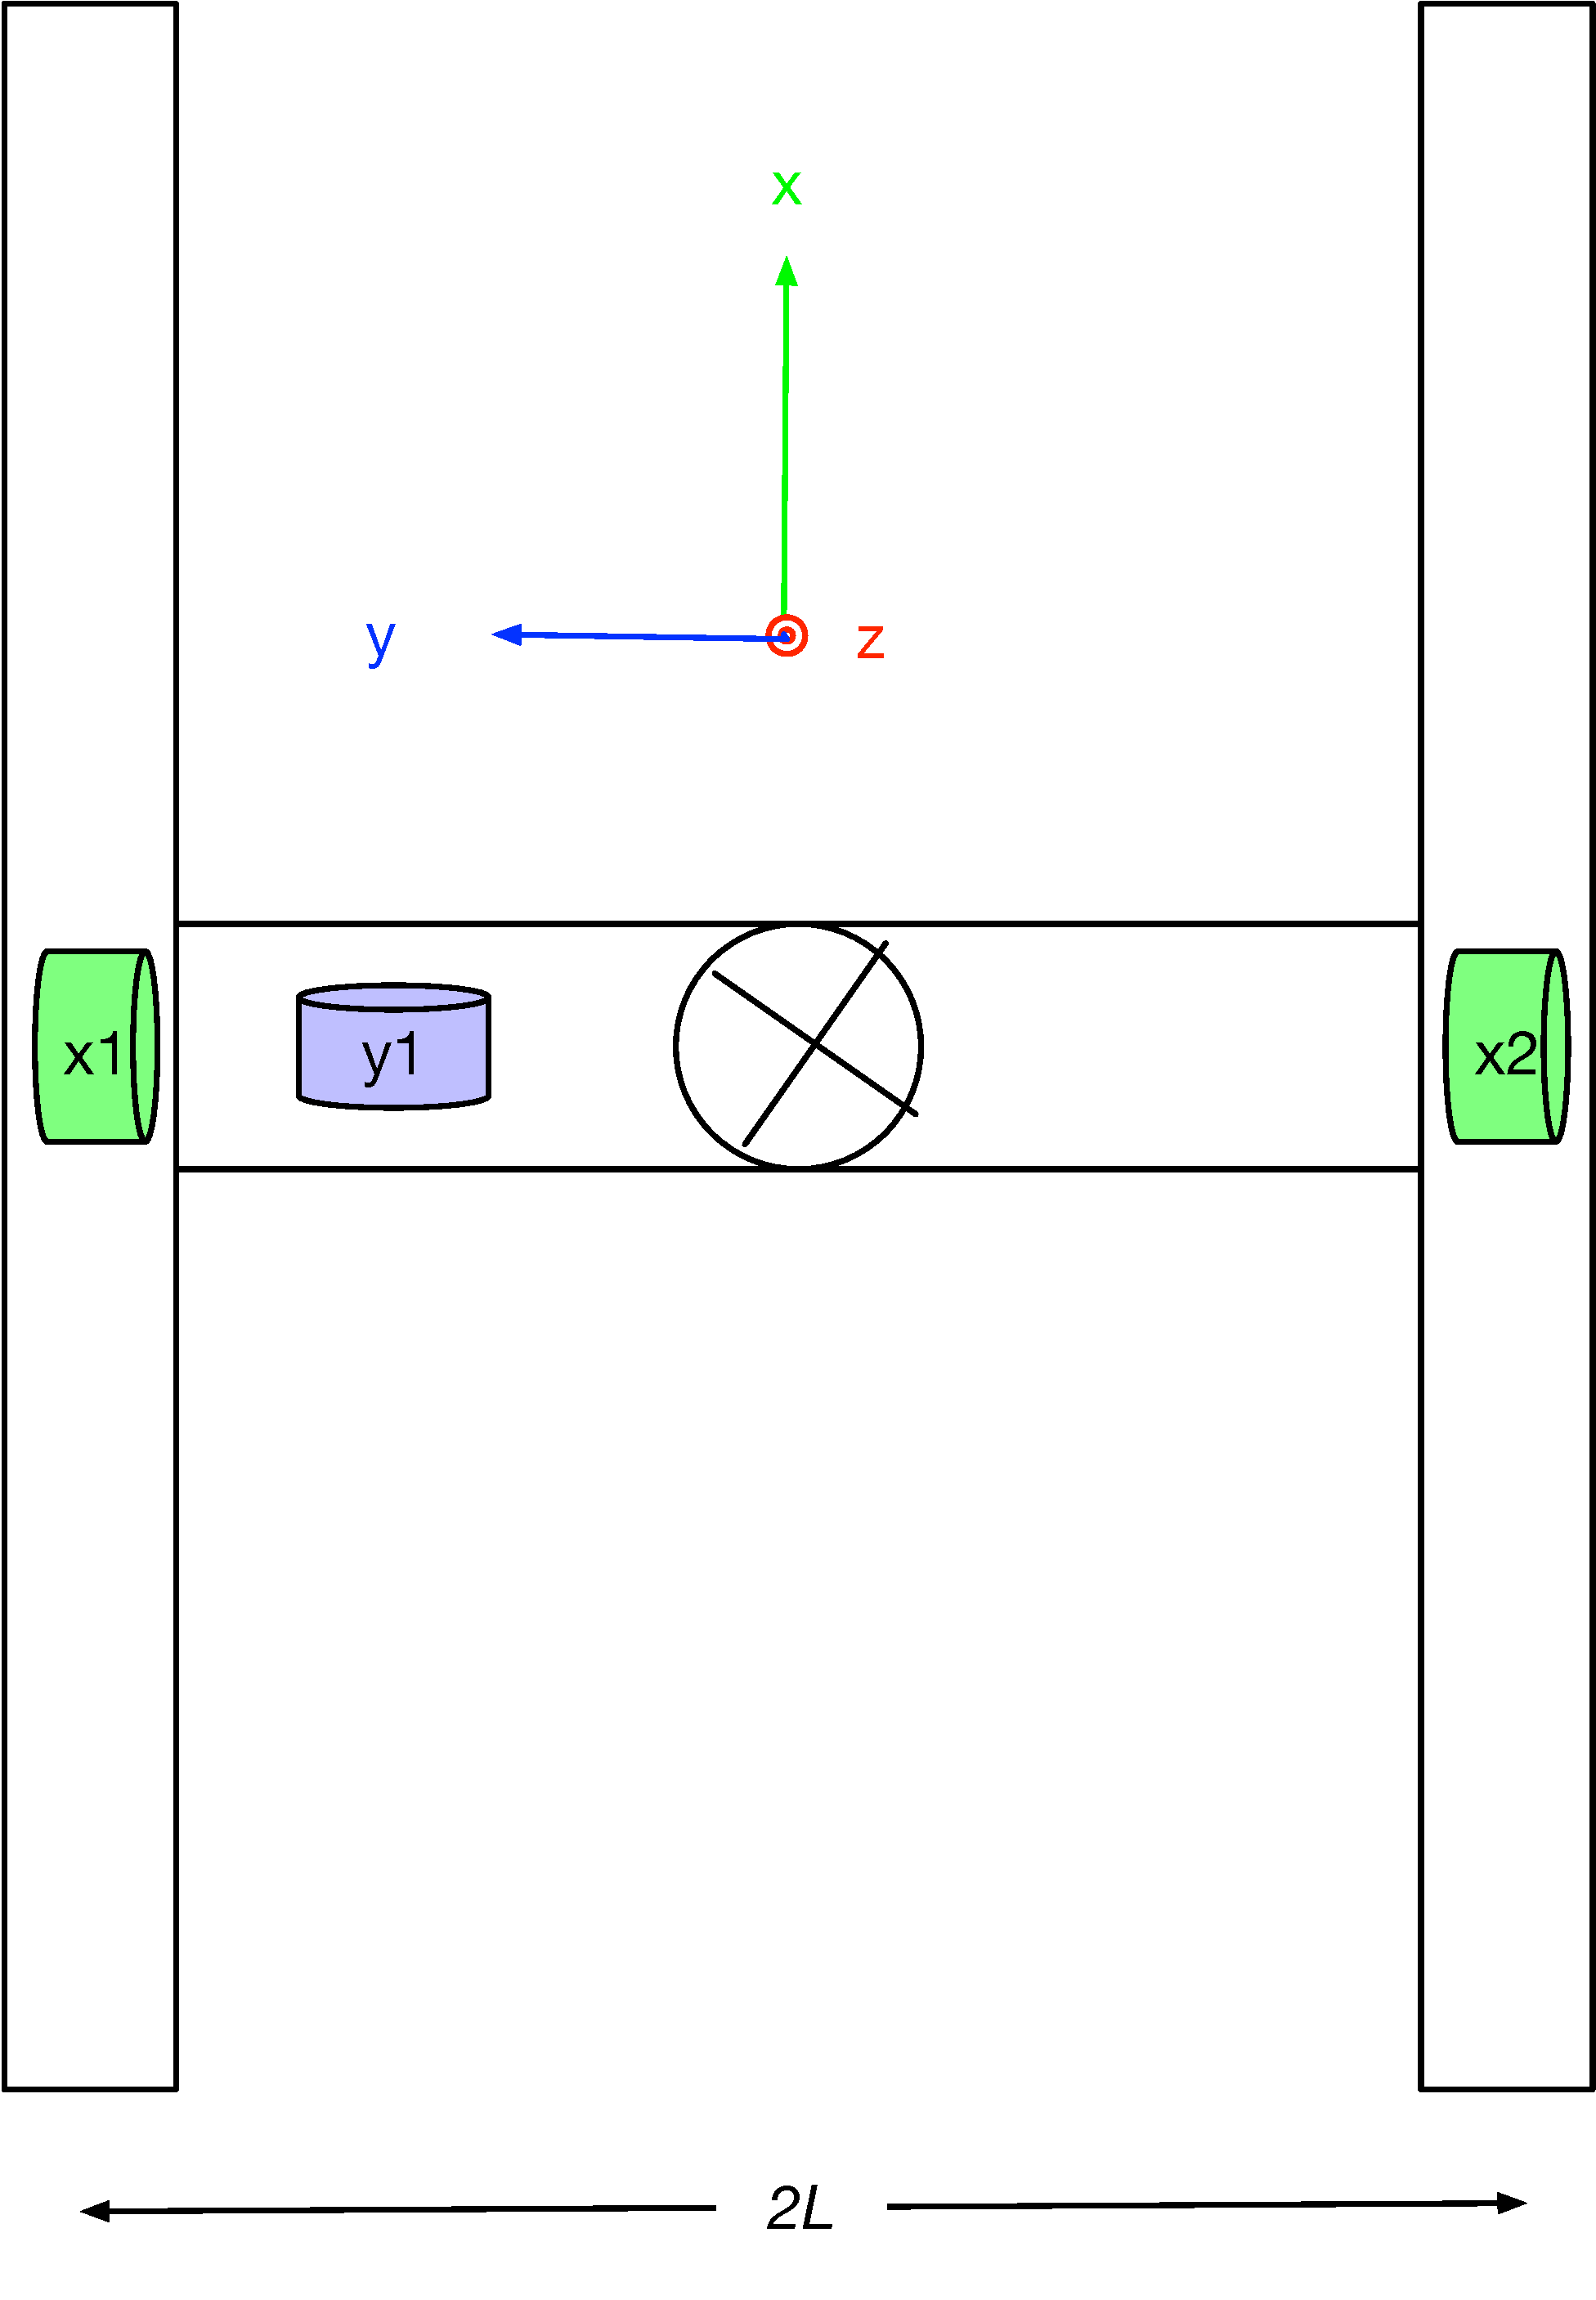
\includegraphics[keepaspectratio,width=1.5in,height=0.75\textheight]{robot_frame}
\caption{Robot Frame of Reference}
\label{robot_frame}
\end{figure}

\begin{itemize}
\item Coordinate Axes

\begin{itemize}
\item \(\hat{x}\): forward

\item \(\hat{y}\): left

\item \(\hat{z}\): up

\end{itemize}

\item Encoders

\begin{itemize}
\item \textbf{x1} and \textbf{x2}: forward and aft

\item \textbf{y1}: side to side

\end{itemize}

\item Measured variables

\begin{itemize}
\item \(R_0\): radius of encoder wheel

\item \(N_0\): number of ``ticks'' per encoder wheel rotation

\item \(N_{x_1}, N_{x_2}, N_{y_1}\): number of ``ticks'' recorded on each encoder

\end{itemize}

\item Computed values

\begin{itemize}
\item \(\Delta N_{x_1}, \Delta N_{x_2}, \Delta N_{y_1}\): number of tickets measured on each encoder during time step

\item \(\Delta s_x, \Delta s_y\): distance measured in forward and left direction in robot frame of reference during time step

\item \(\Delta \theta\): Change in robot heading during time step

\end{itemize}

\end{itemize}

\subsection{Field Frame of Reference}
\label{fieldframeofreference}

\begin{figure}[htbp]
\centering
\includegraphics[keepaspectratio,width=3.5in,height=0.75\textheight]{field_for}
\caption{Field Frame of Reference}
\label{field_for}
\end{figure}

\begin{itemize}
\item Coordinate Axes

\begin{itemize}
\item Origin defined for each game and alliance-specific

\item \(\hat{X}_F\): to right from origin

\item \(\hat{Y}_F\): away from origin

\item \(\theta\): robot heading; clockwise angle from \(\hat{Y}_F\) to \(\hat{x}\):

\end{itemize}

\item Robot Starting Position: \((\hat{X}_{F_0}, \hat{Y}_{F_0}, \theta_{0})\)

\end{itemize}

\section{Time Step}
\label{timestep}

\subsection{Definitions}
\label{definitions}

\begin{itemize}
\item Each time step is an arbitrary amount of time within which robot identifies its location, determines trajectory to objective, and commands motors to follow trajectory

\item Time step duration: \(\Delta t\)

\item Time step starts at: \(t - \Delta t\)

\item Time step ends at: \(t\)

\end{itemize}

\subsection{Activities During Each Time Step}
\label{activitiesduringeachtimestep}

\subsubsection{Navigation (Determine robot location)}
\label{navigationdeterminerobotlocation}

\begin{itemize}
\item Measure each encoder's tick counter at end of time step: \([N_{x_1} (t), N_{x_2} (t), N_{y_1} (t)]\)

\item Compute change in each encoder's tick counter over time step:
\[\Delta N_{x_1} = N_{x_1} (t) - N_{x_1} (t - \Delta t)\]
\[\Delta N_{x_2} = N_{x_2} (t) - N_{x_2} (t - \Delta t)\]
\[\Delta N_{y_1} = N_{y_1} (t) - N_{y_1} (t - \Delta t)\]

\item Compute change in position and heading in robot Frame of Reference
\[\Delta s_x = \frac{R_0}{N_0} \left( \frac{\Delta N_{x_1} + \Delta N_{x_2}}{2} \right)\]
\[\Delta s_y = \frac{R_0}{N_0} \Delta N_{y_1}\]

\item Compute change in position in field Frame of Reference
\[\Delta X_F = \Delta s_x [\sin{\theta (t - \Delta t)}] - \Delta s_y [\cos{\theta (t - \Delta t)]}\]
\[\Delta Y_F = \Delta s_x [\cos{\theta (t - \Delta t)}] + \Delta s_y [\sin{\theta (t - \Delta t)]}\]

\item Compute change in heading
\[\Delta \theta = \frac{R_0}{N_0} \left( \frac{\Delta N_{x_1} - \Delta N_{x_2}}{2L} \right)\]

\item Update robot postion and heading
\[X_F(t) = X_F(t - \Delta t) + \Delta X_F\]
\[Y_F(t) = Y_F(t - \Delta t) + \Delta Y_F\]
\[\theta (t) = \theta (t - \Delta t) + \Delta \theta \]

\end{itemize}

\subsubsection{Guidance (Determine trajectory to designated target)}
\label{guidancedeterminetrajectorytodesignatedtarget}

\subsubsection{Control (Command motors to execute guidance)}
\label{controlcommandmotorstoexecuteguidance}

\begin{itemize}
\item Point and Shoot Technique

\item Strafe Technique

\end{itemize}

\input{mmd6-article-footer}
\end{document}
